\documentclass{article}
\usepackage{amsmath}
\usepackage{amssymb}
\usepackage{graphicx}
\usepackage{hyperref}
\usepackage[version=4]{mhchem}


\begin{document}
Show that for right triangle, if \(\angle A=30^{\circ}\), then \(B C=\frac{1}{2} A B\).

Proof:
Draw the median \(M C\). Since \(M C\) is the median, \(M C=\) \(A M=M B\).\\
\centering
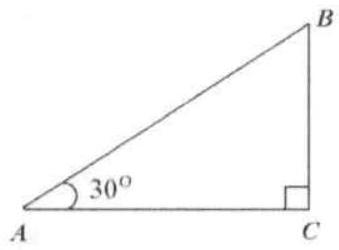
\includegraphics[width=\textwidth]{images/009(4).jpg}

Triangle \(A M C\) is an isosceles triangle with \(\angle M A C=\angle M C A=30^{\circ}\).

Since \(\angle B M C\) is the exterior angle of triangle \(A M C\), \(\angle B M C=\angle M A C+\angle M C A=30^{\circ}+30^{\circ}=60^{\circ}\).\\
So, triangle \(M B C\) is an equilateral triangle with \(B C=\) \(M C=M B\).\\
That is \(B C=\frac{1}{2} A B\).\\
\centering
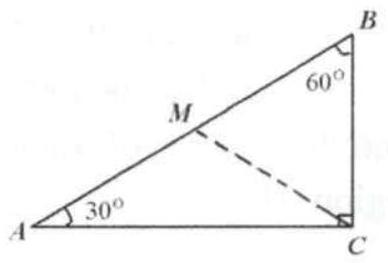
\includegraphics[width=\textwidth]{images/009(3).jpg}


\end{document}
